\documentclass[a4paper,12pt]{article}

\usepackage{my_pkg}
\usepackage{my_pkg2}

\title{Project 7: Using Aggregations as Derived Attributes}
\SetDocumentFooter{}{}

\begin{document}

\maketitle

\section{Objectives}

\myparagraph{In this assignment you look to address scalability concerns with your previous sketches by using aggregation techniques. Again, take care to use good software engineering practices. }

\section{Ground Rules}

\groundrules



\section{Assignment Instructions}

\begin{itemize}

\item Download the data set at \url{
http://www.calvin.edu/~stob/data/srsatact.csv}. This dataset contains standardized scores for all Calvin College 2004 seniors that have taken both the ACT and the SAT, together with their GPAs. There are 271 data points and 4 dimensions.

\item Using your existing dashboard implementation, you will add a few new visualizations (you can remove old ones of your choice).

\item Create a Histogram\footnote{\url{https://en.wikipedia.org/wiki/Histogram}} for each attribute and display using small multiples.

\item Calculate the mean and standard deviation and add them using additional visual encodings.

\item Calculate the Pearson Correlation Coefficient\footnote{\url{http://en.wikipedia.org/wiki/Pearson_correlation}} and Spearman's rank correlation coefficient\footnote{\url{https://en.wikipedia.org/wiki/Spearman\%27s_rank_correlation_coefficient}} for all combination of attributes and show it using a Corrgram (see below for 4 examples of Corrgram). Try to pick a variety beyond just a heatmap (i.e. use extra and/or redundant encodings).

\vspace{15pt}
 \hfill
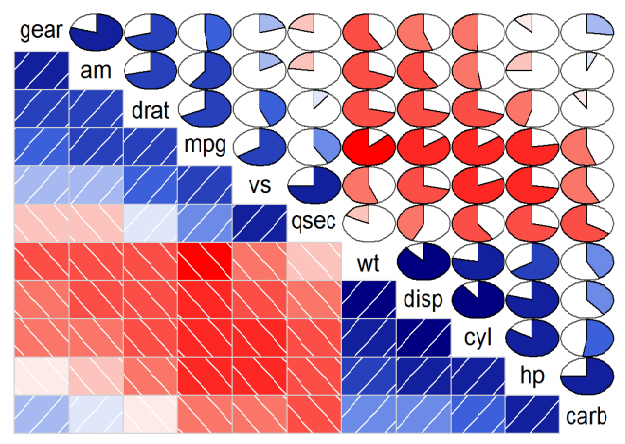
\includegraphics[height=80pt]{images/corrgram1.png} \hfill
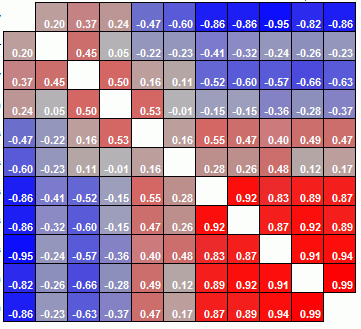
\includegraphics[height=80pt]{images/corrgram2.png} \hfill
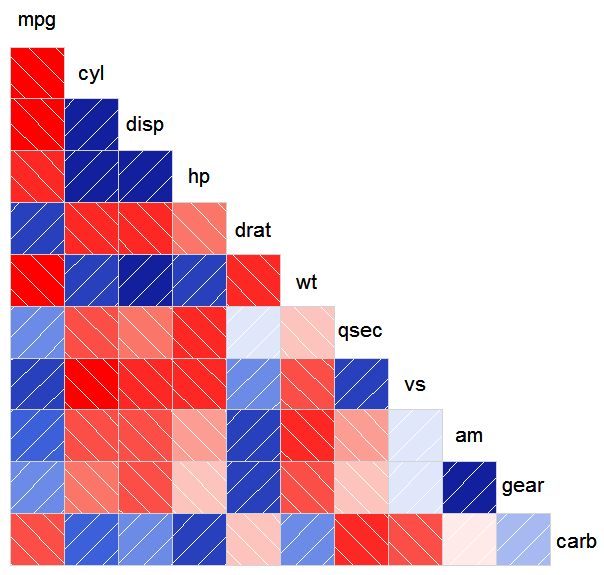
\includegraphics[height=80pt]{images/corrgram3.png} \hfill
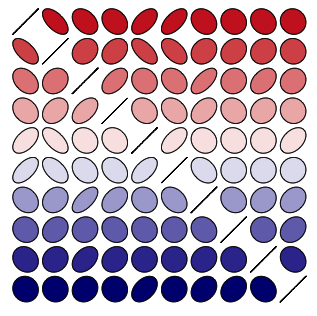
\includegraphics[height=80pt]{images/corrgram4.png} \hfill
\vspace{10pt}

\item Make sure your code works with the Calvin College dataset and at least 1 other dataset from Canvas.

\item Modify your sketch to use any additional linking, interactions, or visual channels to encoding additional variables. Your selection and their implementation will have an impact on your grade.

\item Add embellishments of your choice. These can include but are not limited to: axis lines, labels, and tick marks. Your selection and their implementation will have an impact on your grade.

\item Make sure your visualizations are robust by designing them to support other data (number of elements or value range) and by designing them to support any size of canvas.

\end{itemize}


\section{Submission}

\submission{project7}

\section{Grading and Feedback}

\feedback










\newpage


\begin{center}
{\huge Project 7 Peer Review}
\end{center}




\StartTable{Visual Design}

\AddMultipleChoiceElement{Visual Channels}
	{What visual channels were used to encode data? }
    { 
     \AddMCColumn{1.65cm}{\choice Position	\\ \choice Depth	\\ \choice Angle}
     \AddMCColumn{1.95cm}{\choice Curvature	\\ \choice Shape	\\ \choice Length}
     \AddMCColumn{2.3cm}{\choice Area		\\ \choice Volume  	\\ \choice Luminance/\\\ \ Saturation}
     \AddMCColumn{1.95cm}{\choice Color Hue	\\ \choice Texture	\\ \choice Motion/\\\ \ Animation}
    }
        
\AddElement{Intended/Unintended Encodings}
	{Do all of the visual encoding appear to be intended, or were some accidentally created?}
        {\choice Many\\Unintended}
        {\choice Few\\Unintended}
        {\choice All\\Intended} 
        
\AddElementExtended{Expressiveness of Encodings}
	{Are the visual encodings attached to the correct type of data for that 
    	encoding (i.e.\ are quantitative data attached to quantitative 
        encodings and categorical data to categorical encodings)?}
    {\choice Many\\Errors}
    {\choice Few\\Errors}
    {\choice Correctly\\Assigned} 
            
\AddElement{Effectiveness of Encodings}
	{Have the maximally effective visual encodings been selected in all cases? }
    {\choice Many\\Ineffective}
    {\choice Few\\Ineffective}
    {\choice Most\\Effective} 
        
\AddElement{Effective Use of Color}
	{Is color used in a same fashion? Do the colors chosen and the application 
    	of those colors make the visualization effective?}
    {\choice Mostly\\Ineffective}
    {\choice None\\Used}
    {\choice Highly\\Effective} 

\EndTable  

\vspace{15pt}

\StartTable{Design Considerations}

\AddElement{Clear, Detailed, and Thorough Labeling}
   	{Is appropriate and complete labeling used throughout or do 
      	missing labels require assumptions about the data?}
    {\choice No labels}
    {\choice Some Missing labels}
    {\choice Completely labeled} 
        
\AddElement{Missing Scales}
   	{Are scales provided for the data?}
	{\choice No Scales}
	{\choice Some Missing Scales}
	{\choice All Scales Present} 

\AddElement{Missing Legend}
	{Is a legend provided for the data? Does the legend provide useful 
    	information?}
	{\choice No Legend}
	{\choice Incomplete Legend}
	{\choice Complete Legend} 
        
        
\EndTable  


\StartTable{Design Considerations (cont.)}

\AddElement{Scale Distortion}
	{Is any scale distortion or deception used in the visualization?}	
	{\choice Severe Distortion}
	{\choice Minor Distortion}
	{\choice No Distortion} 
        
\AddElement{Lie Factor}
	{Is there any lie factor? How extreme is the lie factor?}
	{\choice Major Lie}
	{\choice Minor Lie}
	{\choice No Lie} 

\AddElement{Data/Ink Ratio}
	{Is the data to ink ratio reasonable? Could it be more efficient?}
	{Way Too $\square$~Little / $\square$~Much Ink}
	{Slightly Too $\square$~Little / $\square$~Much Ink}
	{\choice Perfect Amount of Ink} 
        
\AddElement{Chart Junk, Embellishments, Aesthetics}
	{Are appropriate embellishments used? Are the embellishments 
    	distracting? Do the embellishments add to the visualization?}
	{Way Too $\square$~Few / $\square$~Many Embellishments}
	{A Bit Too $\square$~Few / $\square$~Many Embellishments}
	{\choice Perfect Number of Embellishments} 
        
\AddElement{Data Density}
	{Has too much data been included in the visualization making 
    	interpretation difficult? } 
	{\choice Too Sparse}
	{\choice Expected}
	{\choice Too Dense} 
        
\AddElement{Gestalt Principals}
	{Have Gestalt principals been used to improve analysis?}
	{\choice No Gestalt Principals}
	{\choice Some Gestalt Principals}
	{\choice Many Gestalt Principals} 
        
\EndTable  
 



\newpage


\begin{center}
{\huge Project 7 Grading}
\end{center}

\begin{itemize}
	\item 2 new visualizations in dashboard - 8 points (4 points each)
	\item Additional interaction, embellishment, and additional Visual Channels - 1.0 points 
		\begin{itemize}
    		\item 0.25 points for none used
    		\item 0.75 point for a few
            \item 1.0 points for many
		\end{itemize}
	\item Code Professionalism - 1.0 points
		\begin{itemize}
            \item 0.25 no comments, no classes, "hard coded" values
            \item 0.75 minimally commented, few "hard coded" values
            \item 1.0 commented, used classes, few "hard coded" values
		\end{itemize}
\end{itemize}



\end{document}




